\section{Question 4}
In this problem we use masserati ghibli data. For cancelling oscillation we use derivative controller to make overshoot low and increase gain to be fast enough with low overshoot.
\begin{center}
    \begin{table}[H]\caption{Maserati ghibli data}
        \centering
        \begin{tabular}{ c c c }
            \hline
            Paramete & Unit & Value \\ 
            \hline
            M & kg & 1900 \\
            $C_d$ & 1 & 0.29\\
            \hline
           \end{tabular}
    \end{table}
\end{center}
In this problem we use 
\newpage
\begin{itemize}
    \item system step responde
    \begin{figure}[H]
        \caption{system step responde}
        \centering
        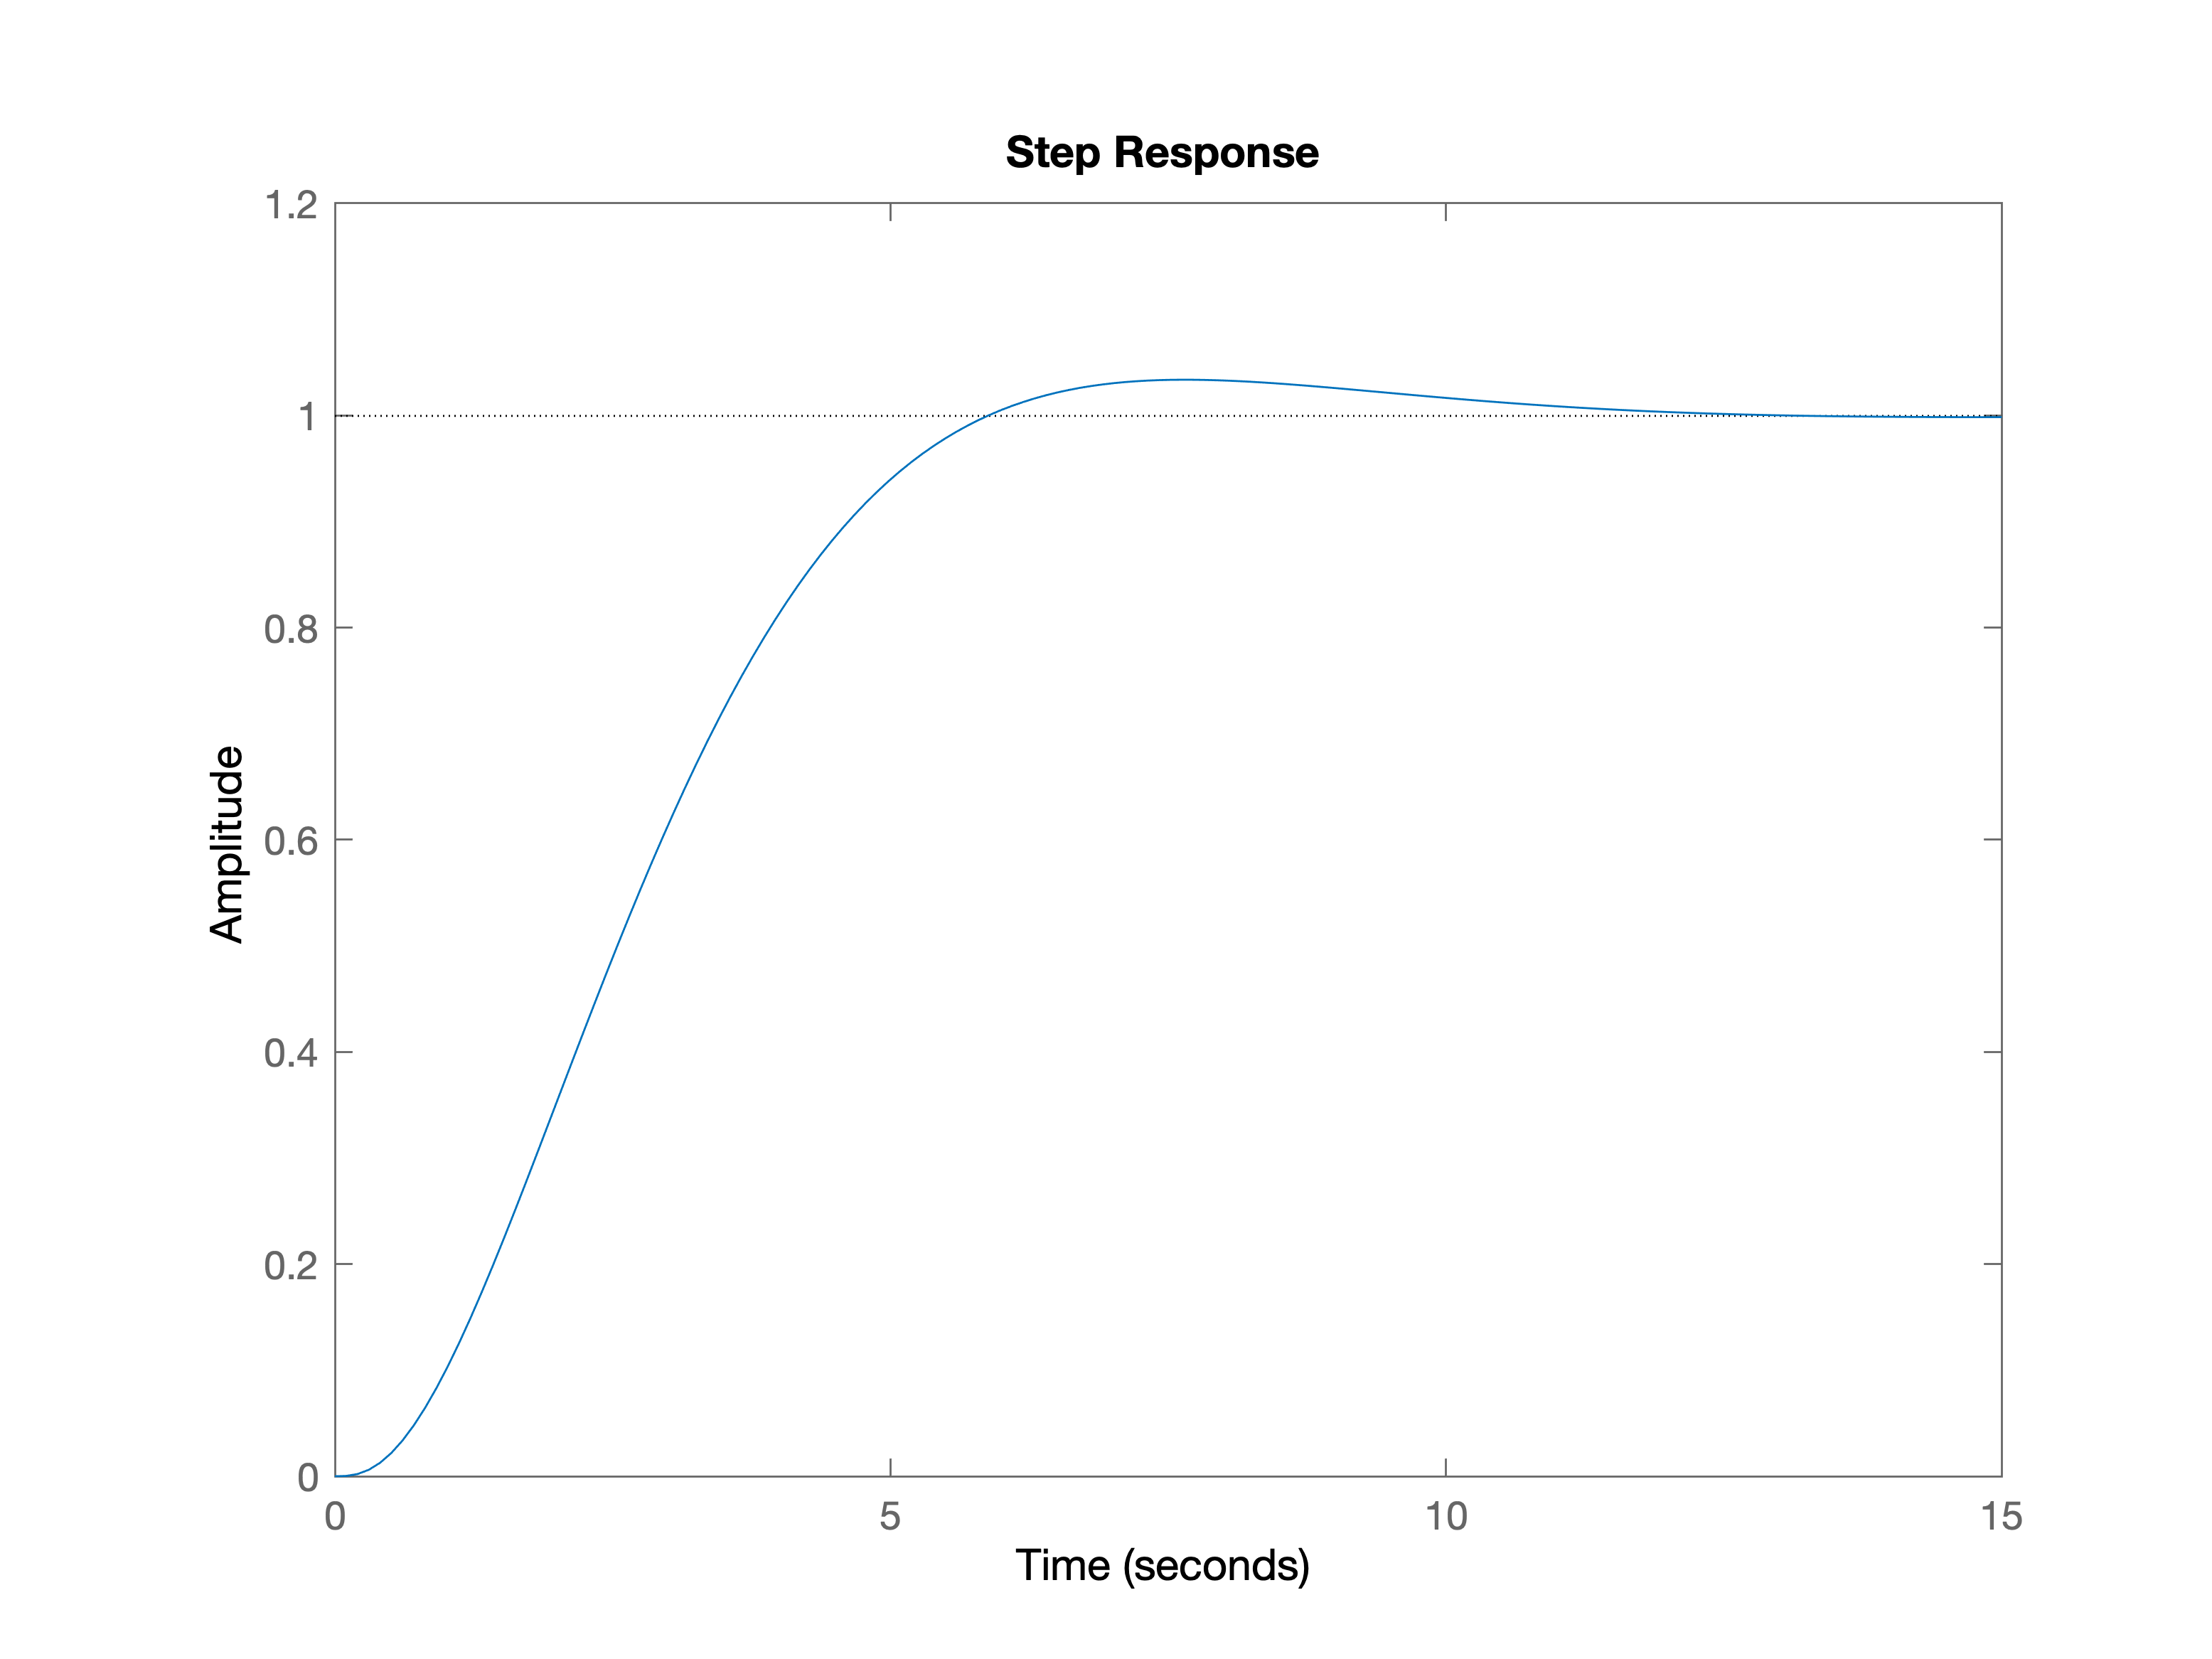
\includegraphics[width=12cm]{../Figure/Q4/Q4_system_respond.png}
    \end{figure}
    \item system rlocus
    \begin{figure}[H]
        \caption{system rlocus plot}
        \centering
        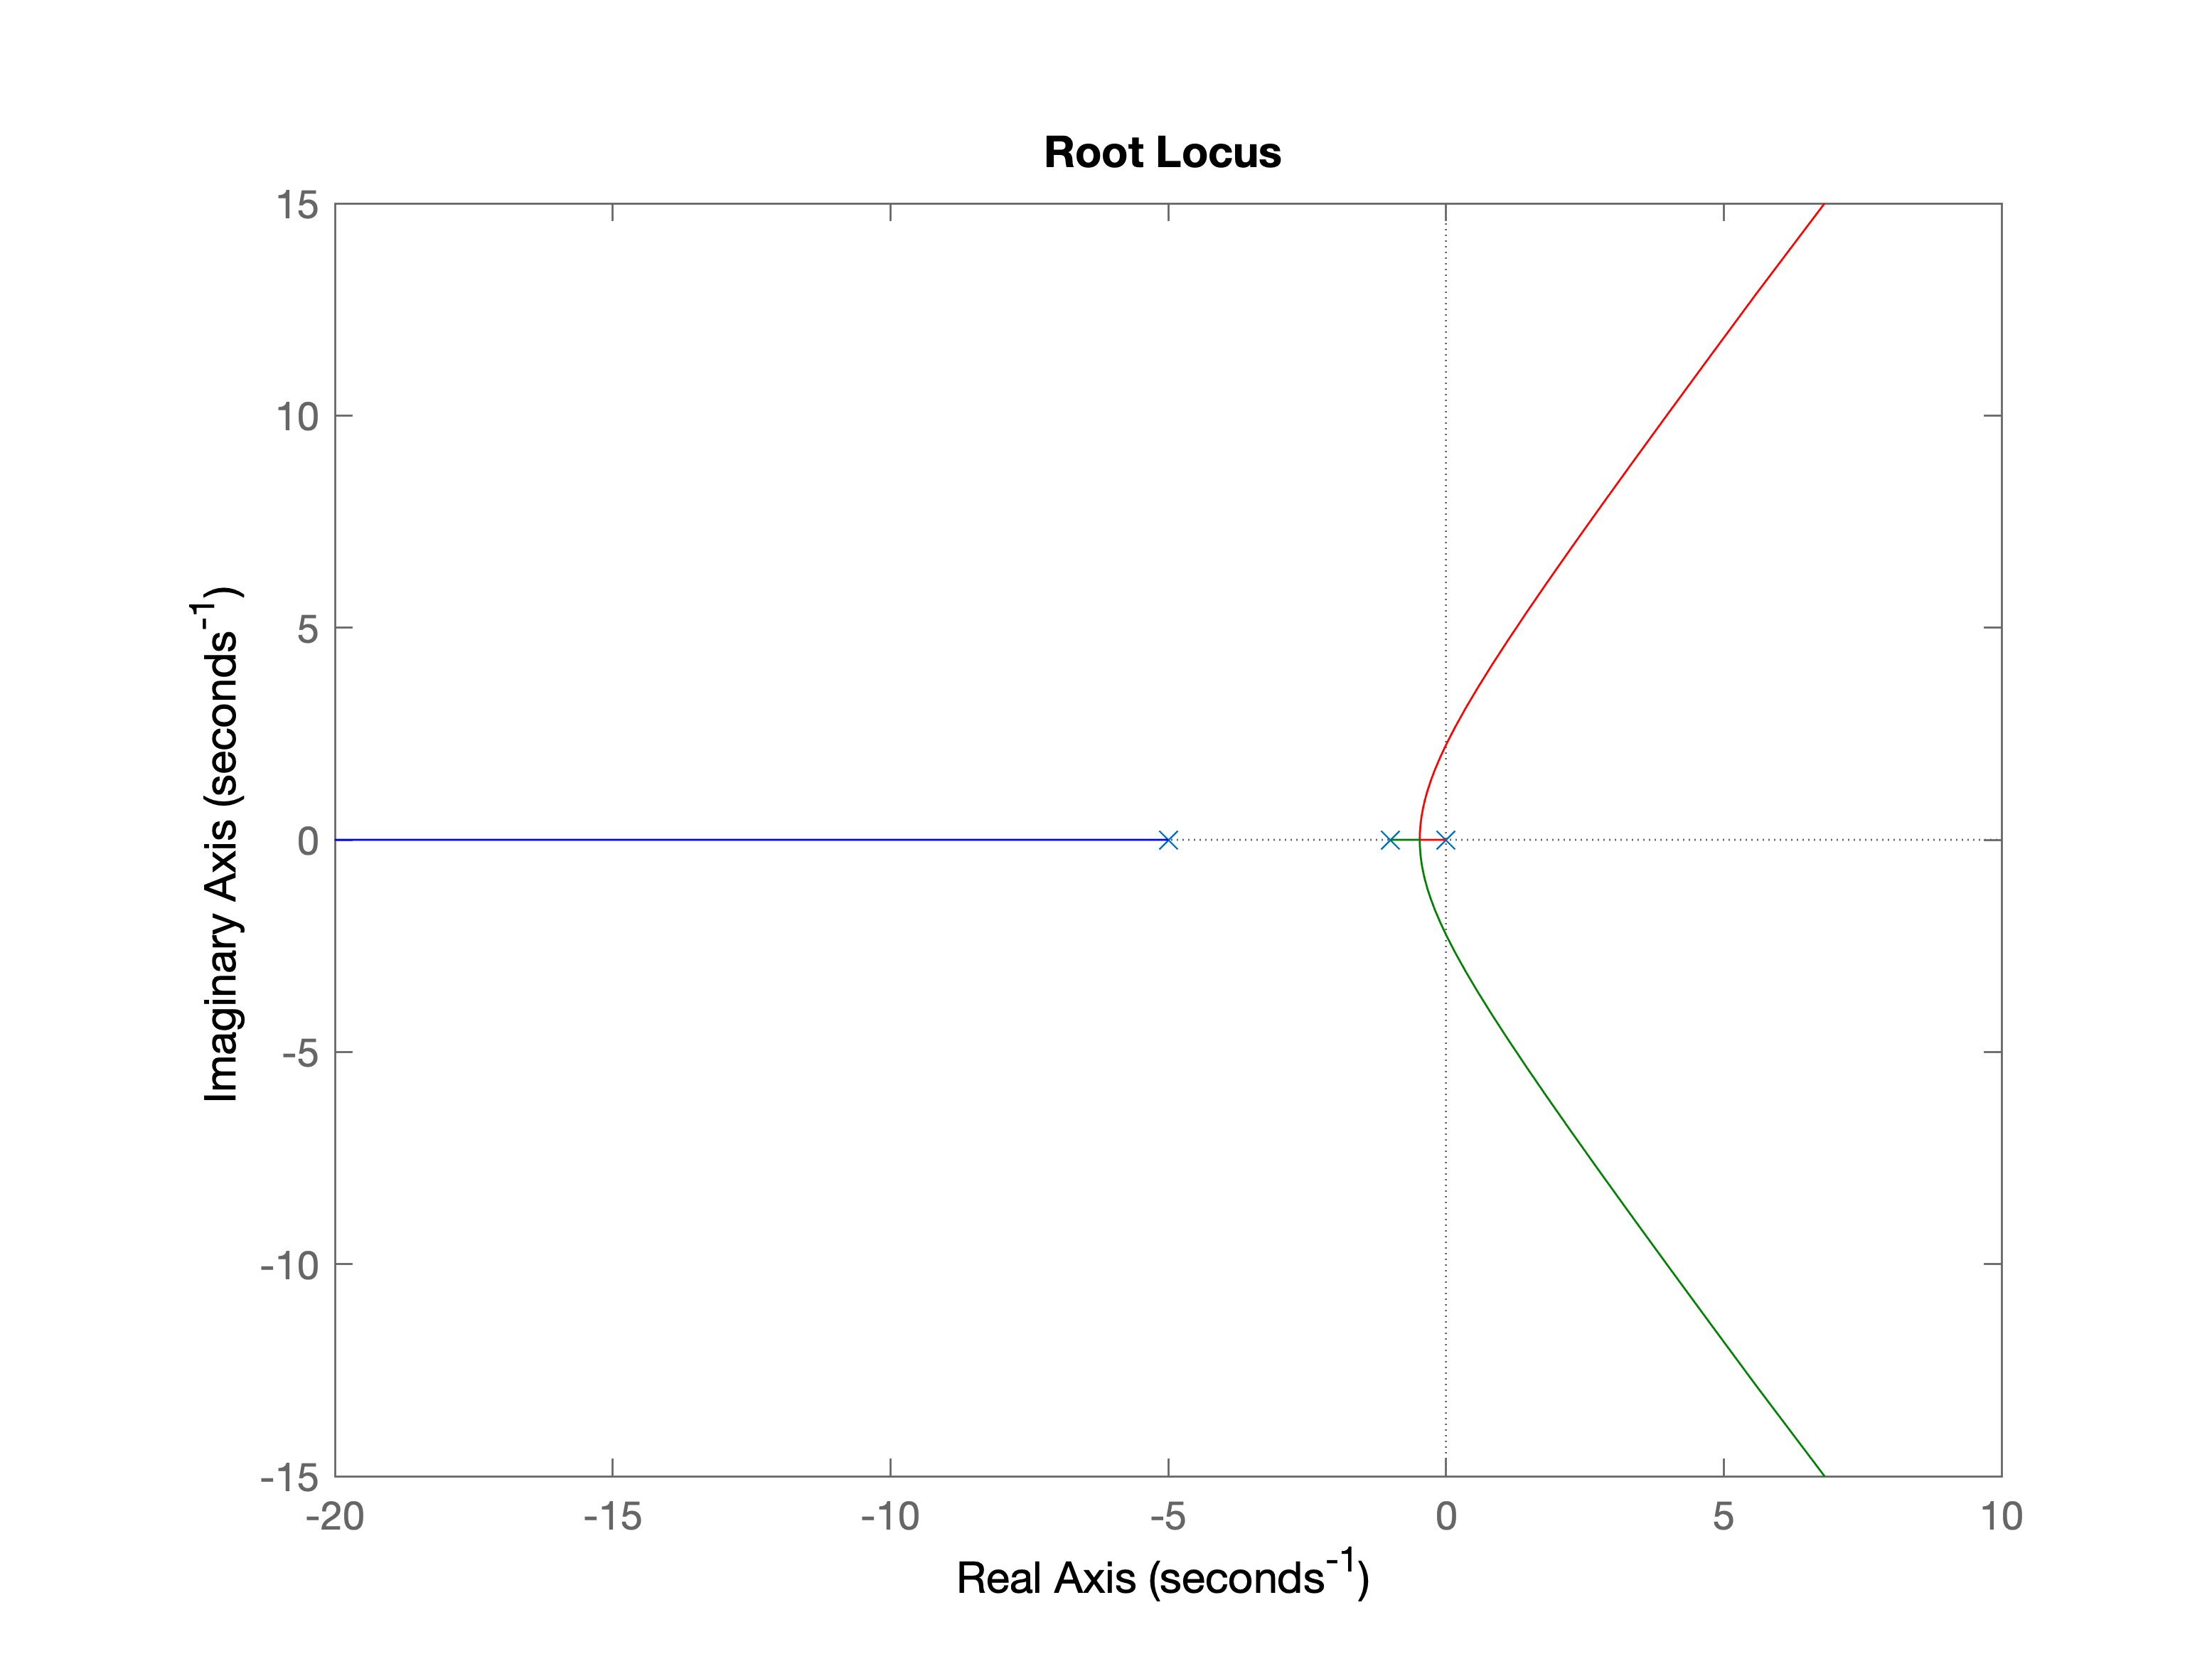
\includegraphics[width=12cm]{../Figure/Q4/Q4_system_rlocus.png}
    \end{figure}
    \item system with controller step responde
    \begin{figure}[H]
        \caption{system with controller step responde}
        \centering
        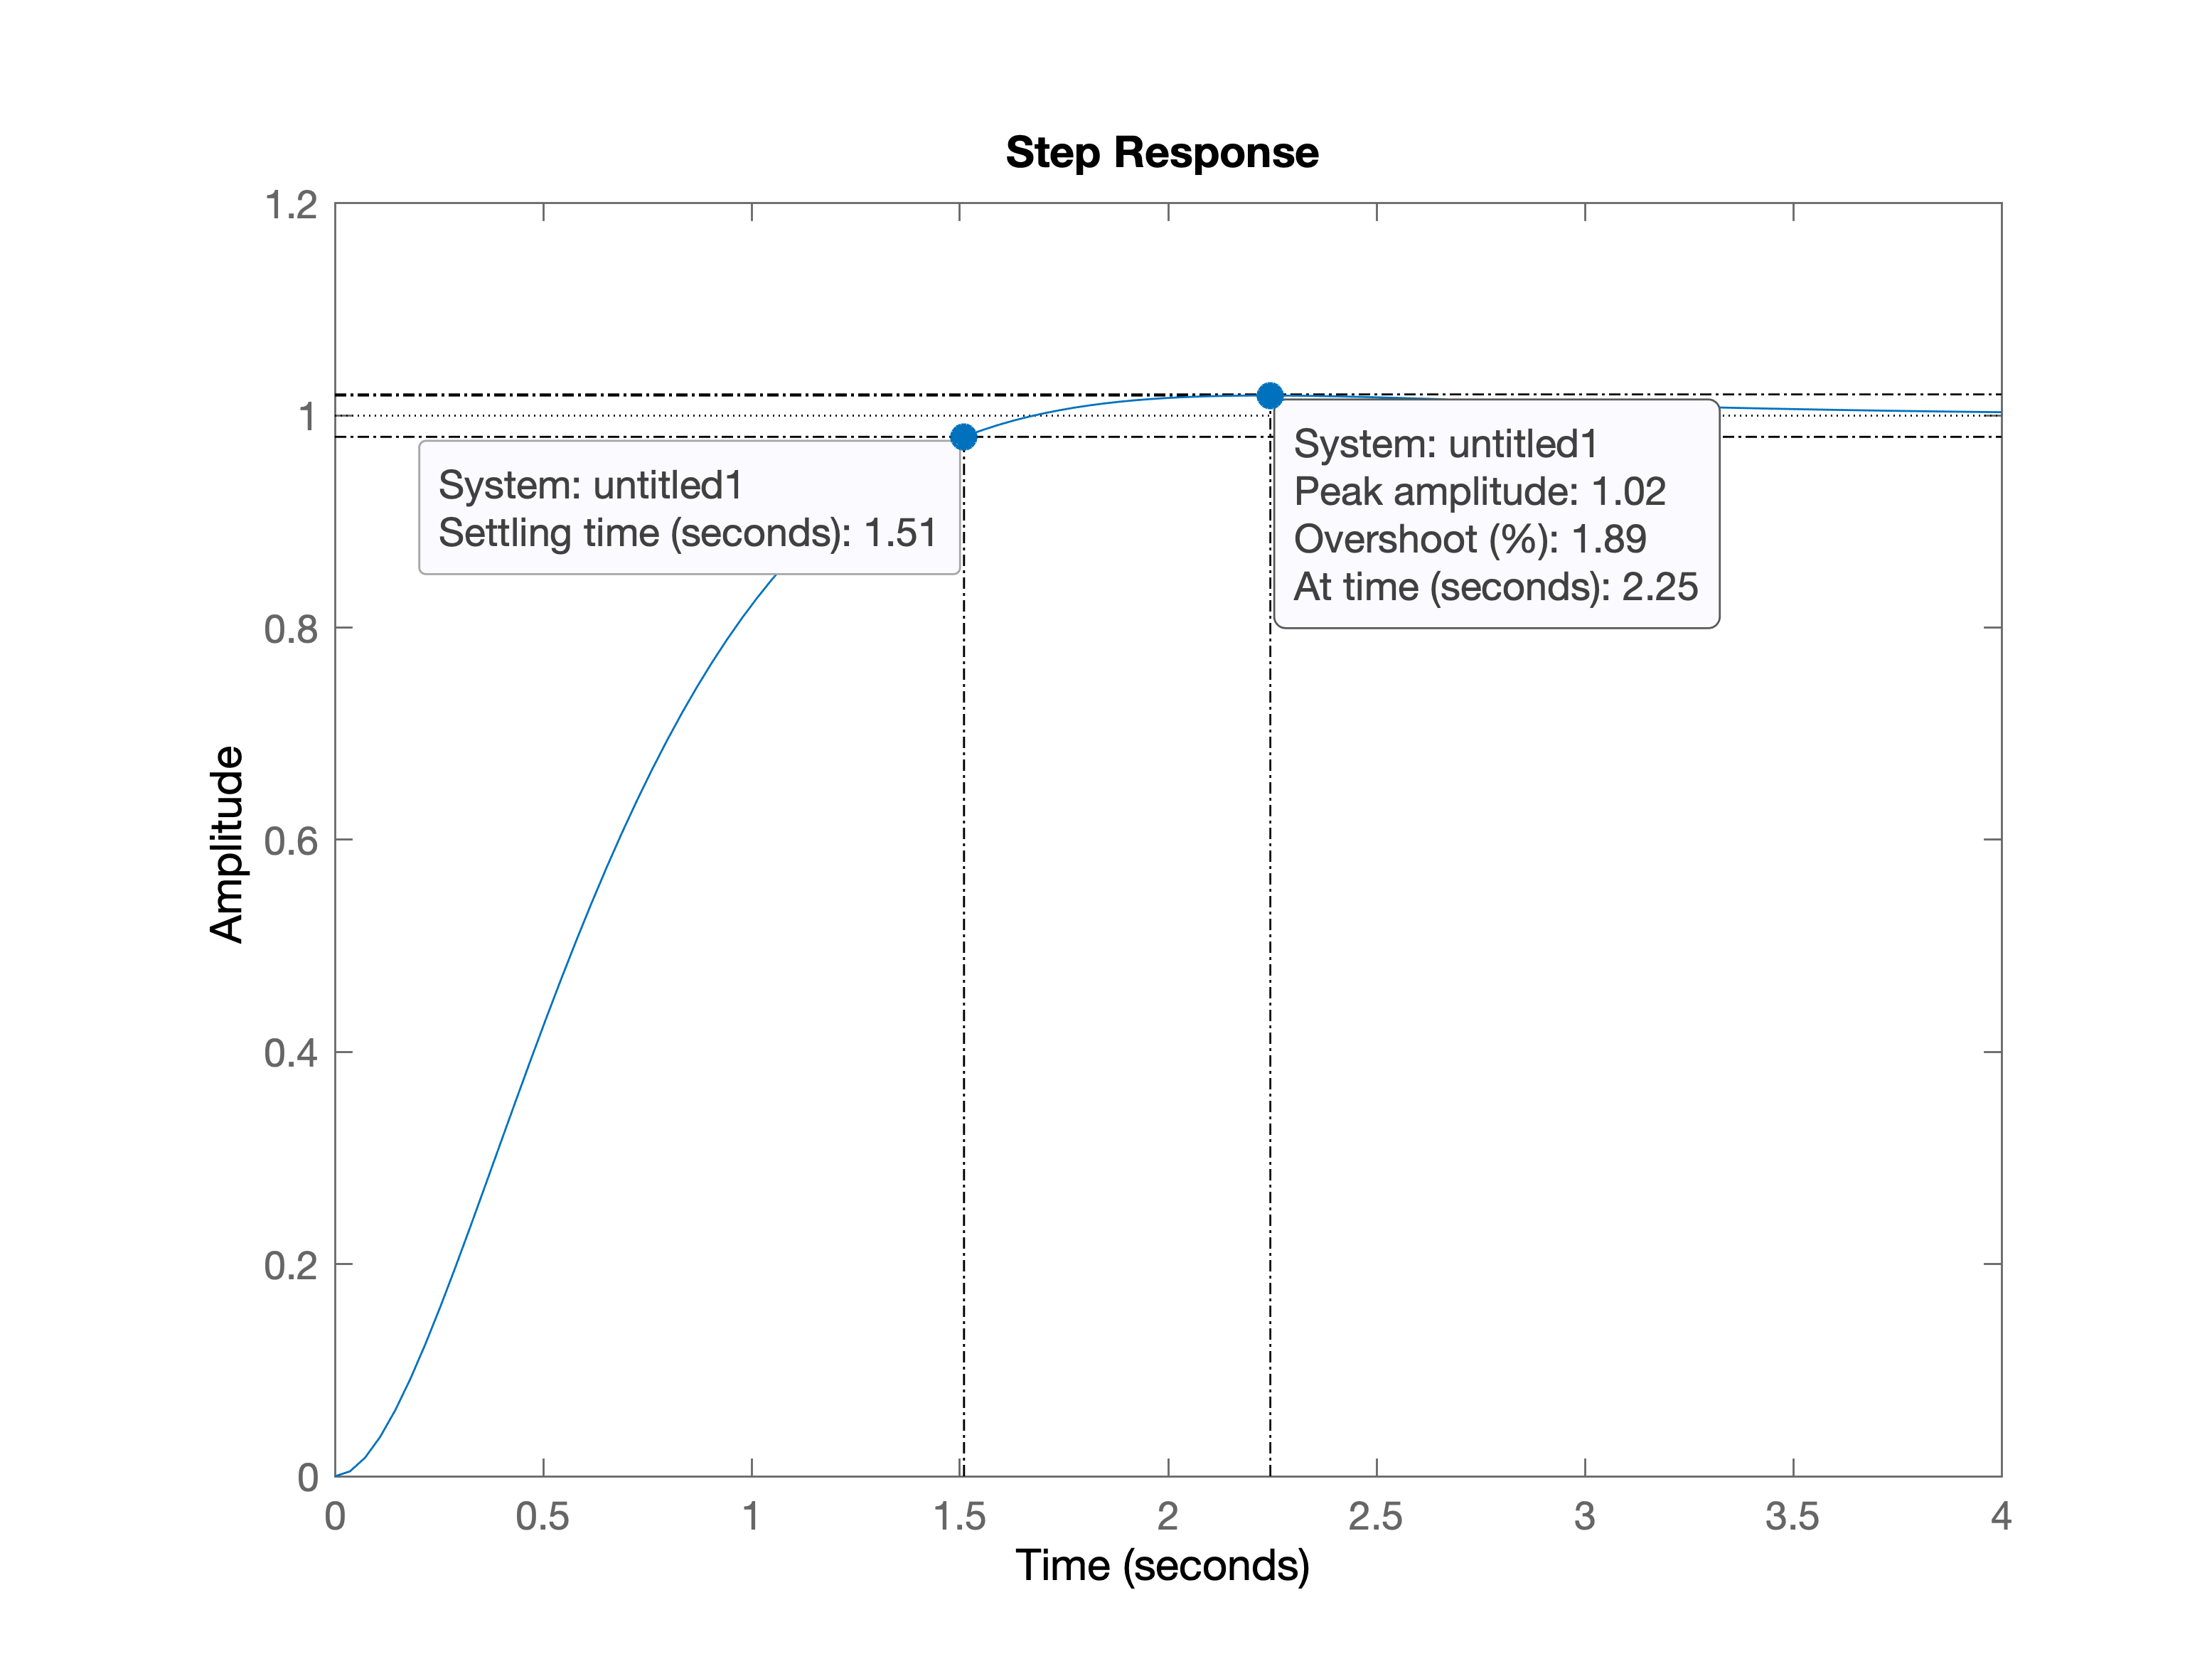
\includegraphics[width=12cm]{../Figure/Q4/Q4_system_controller_respond.png}
    \end{figure}
    \item system with controller rlocus
    \begin{figure}[H]
        \caption{system with controller rlocus plot}
        \centering
        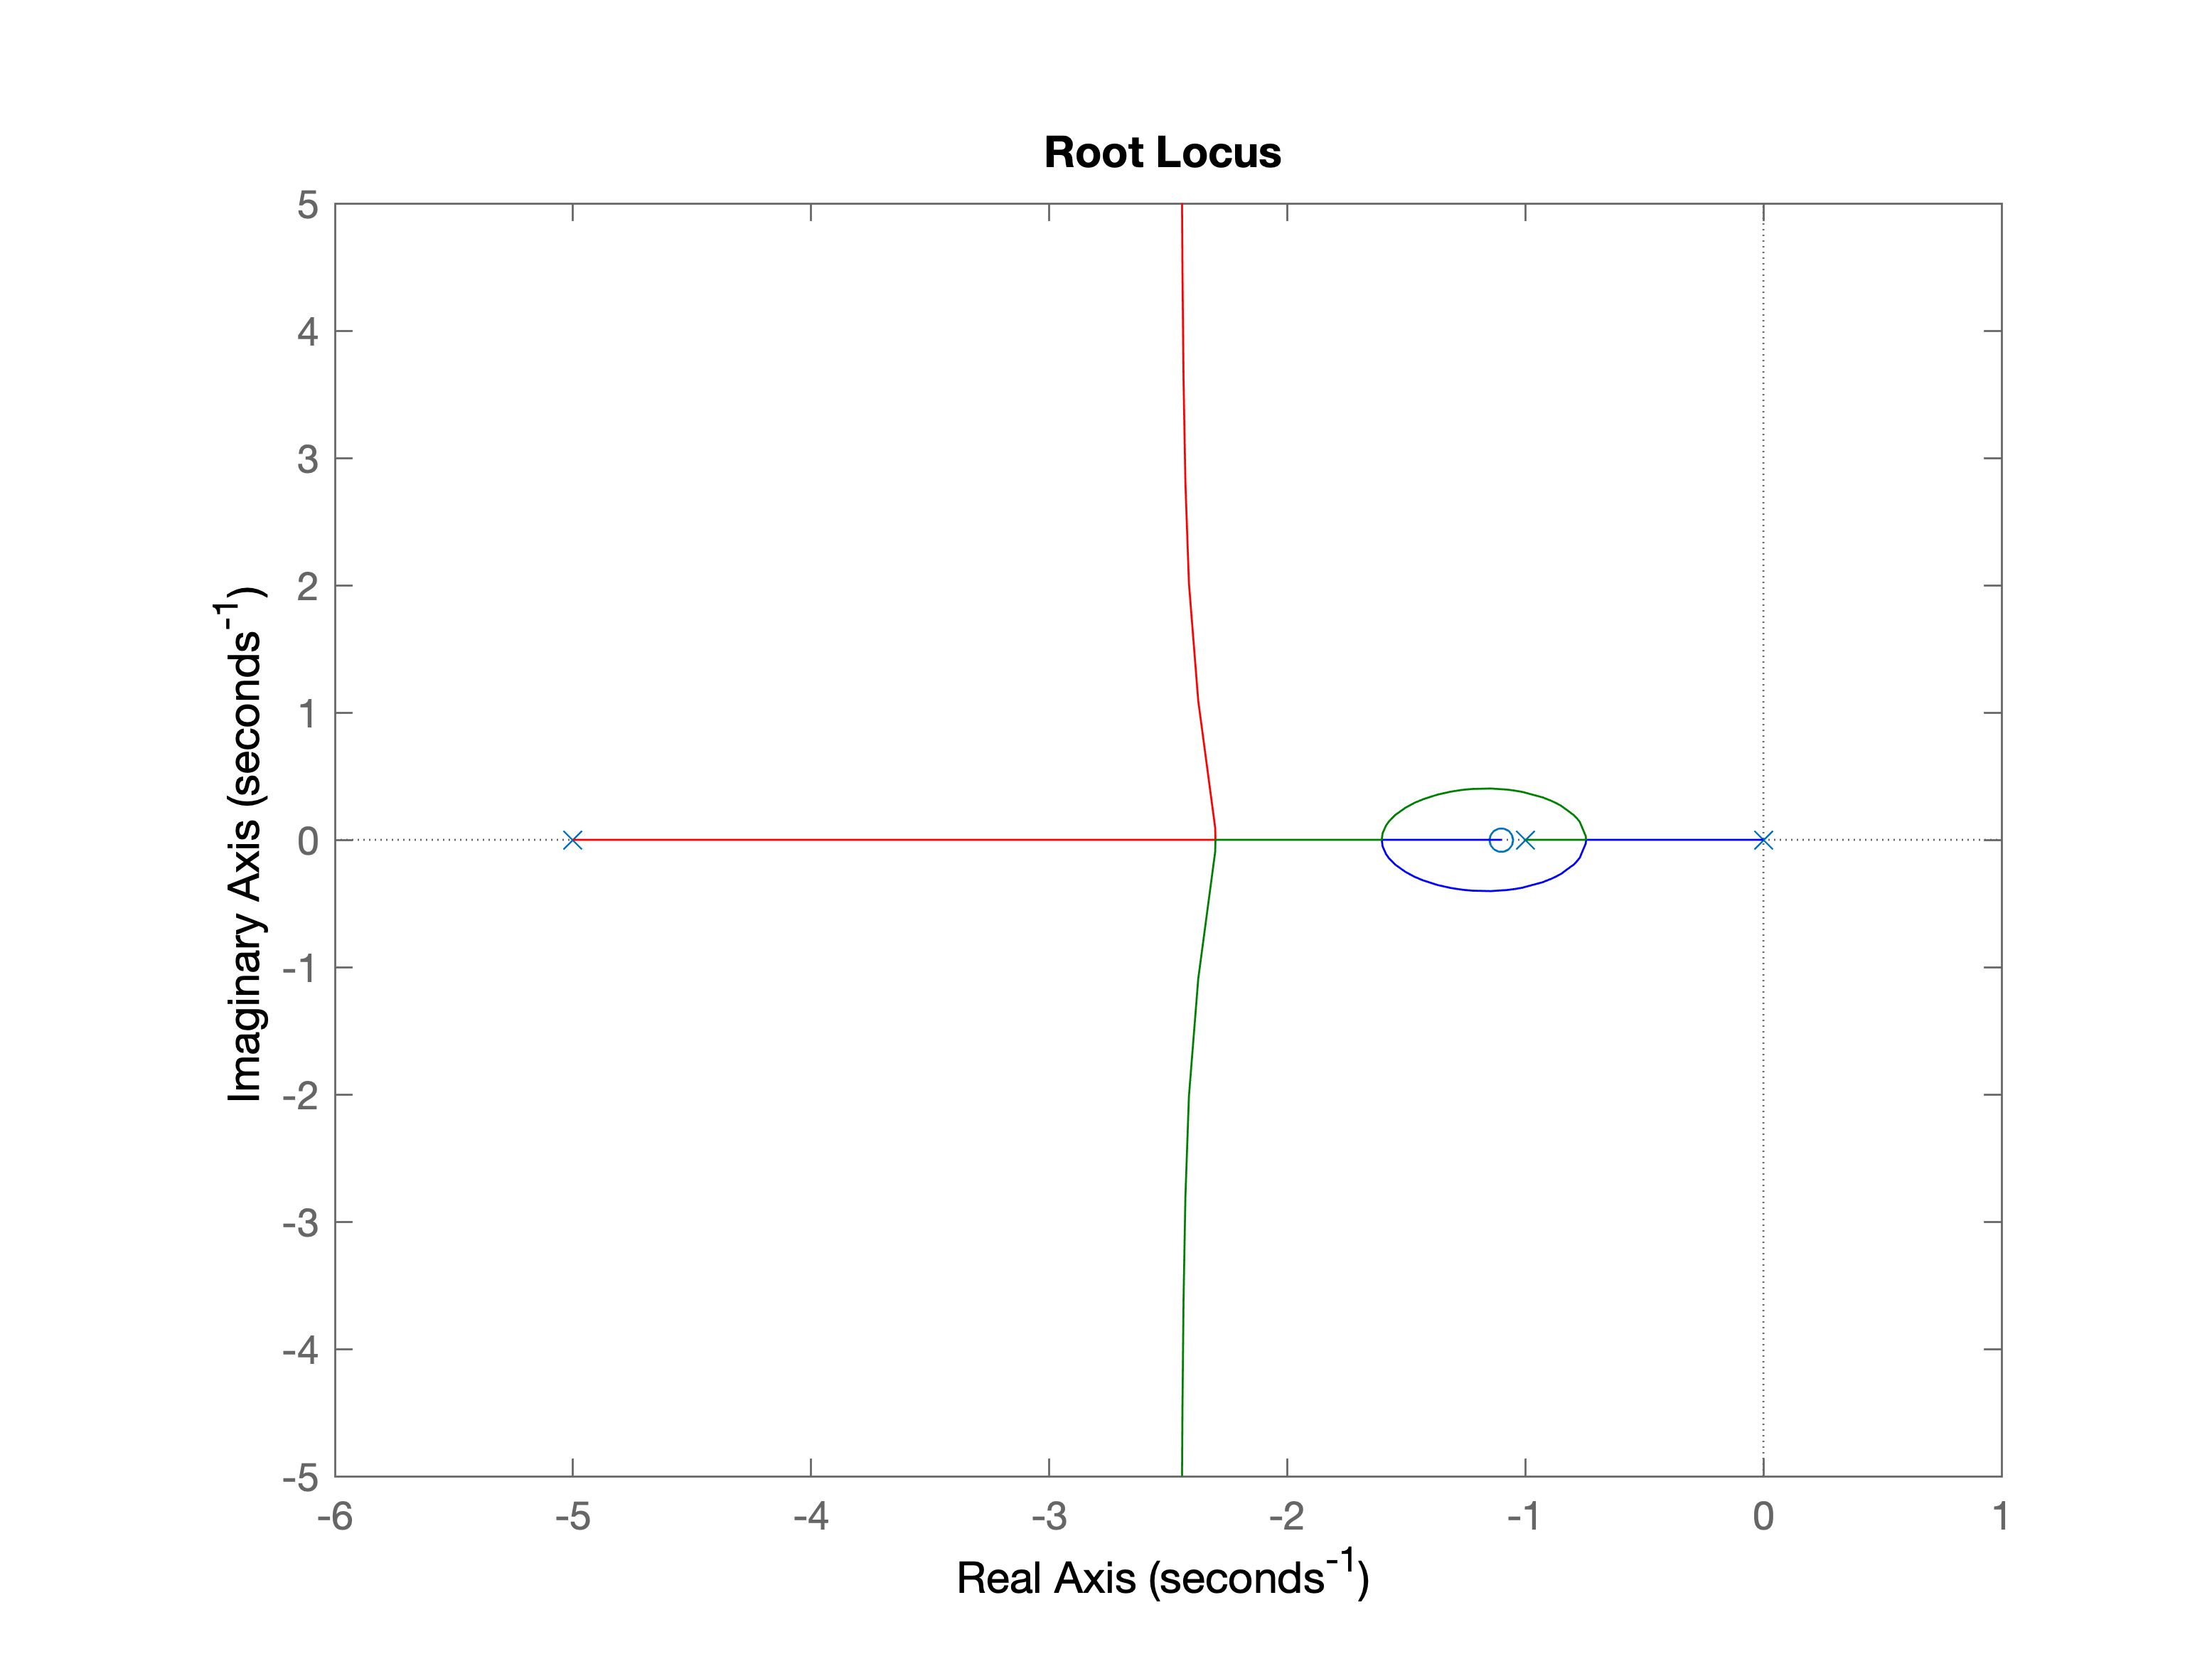
\includegraphics[width=12cm]{../Figure/Q4/Q4_system_controller_rlocus.png}
    \end{figure}
    \item system with and without controller step responde
    \begin{figure}[H]
        \caption{system with and without controller step responde}
        \centering
        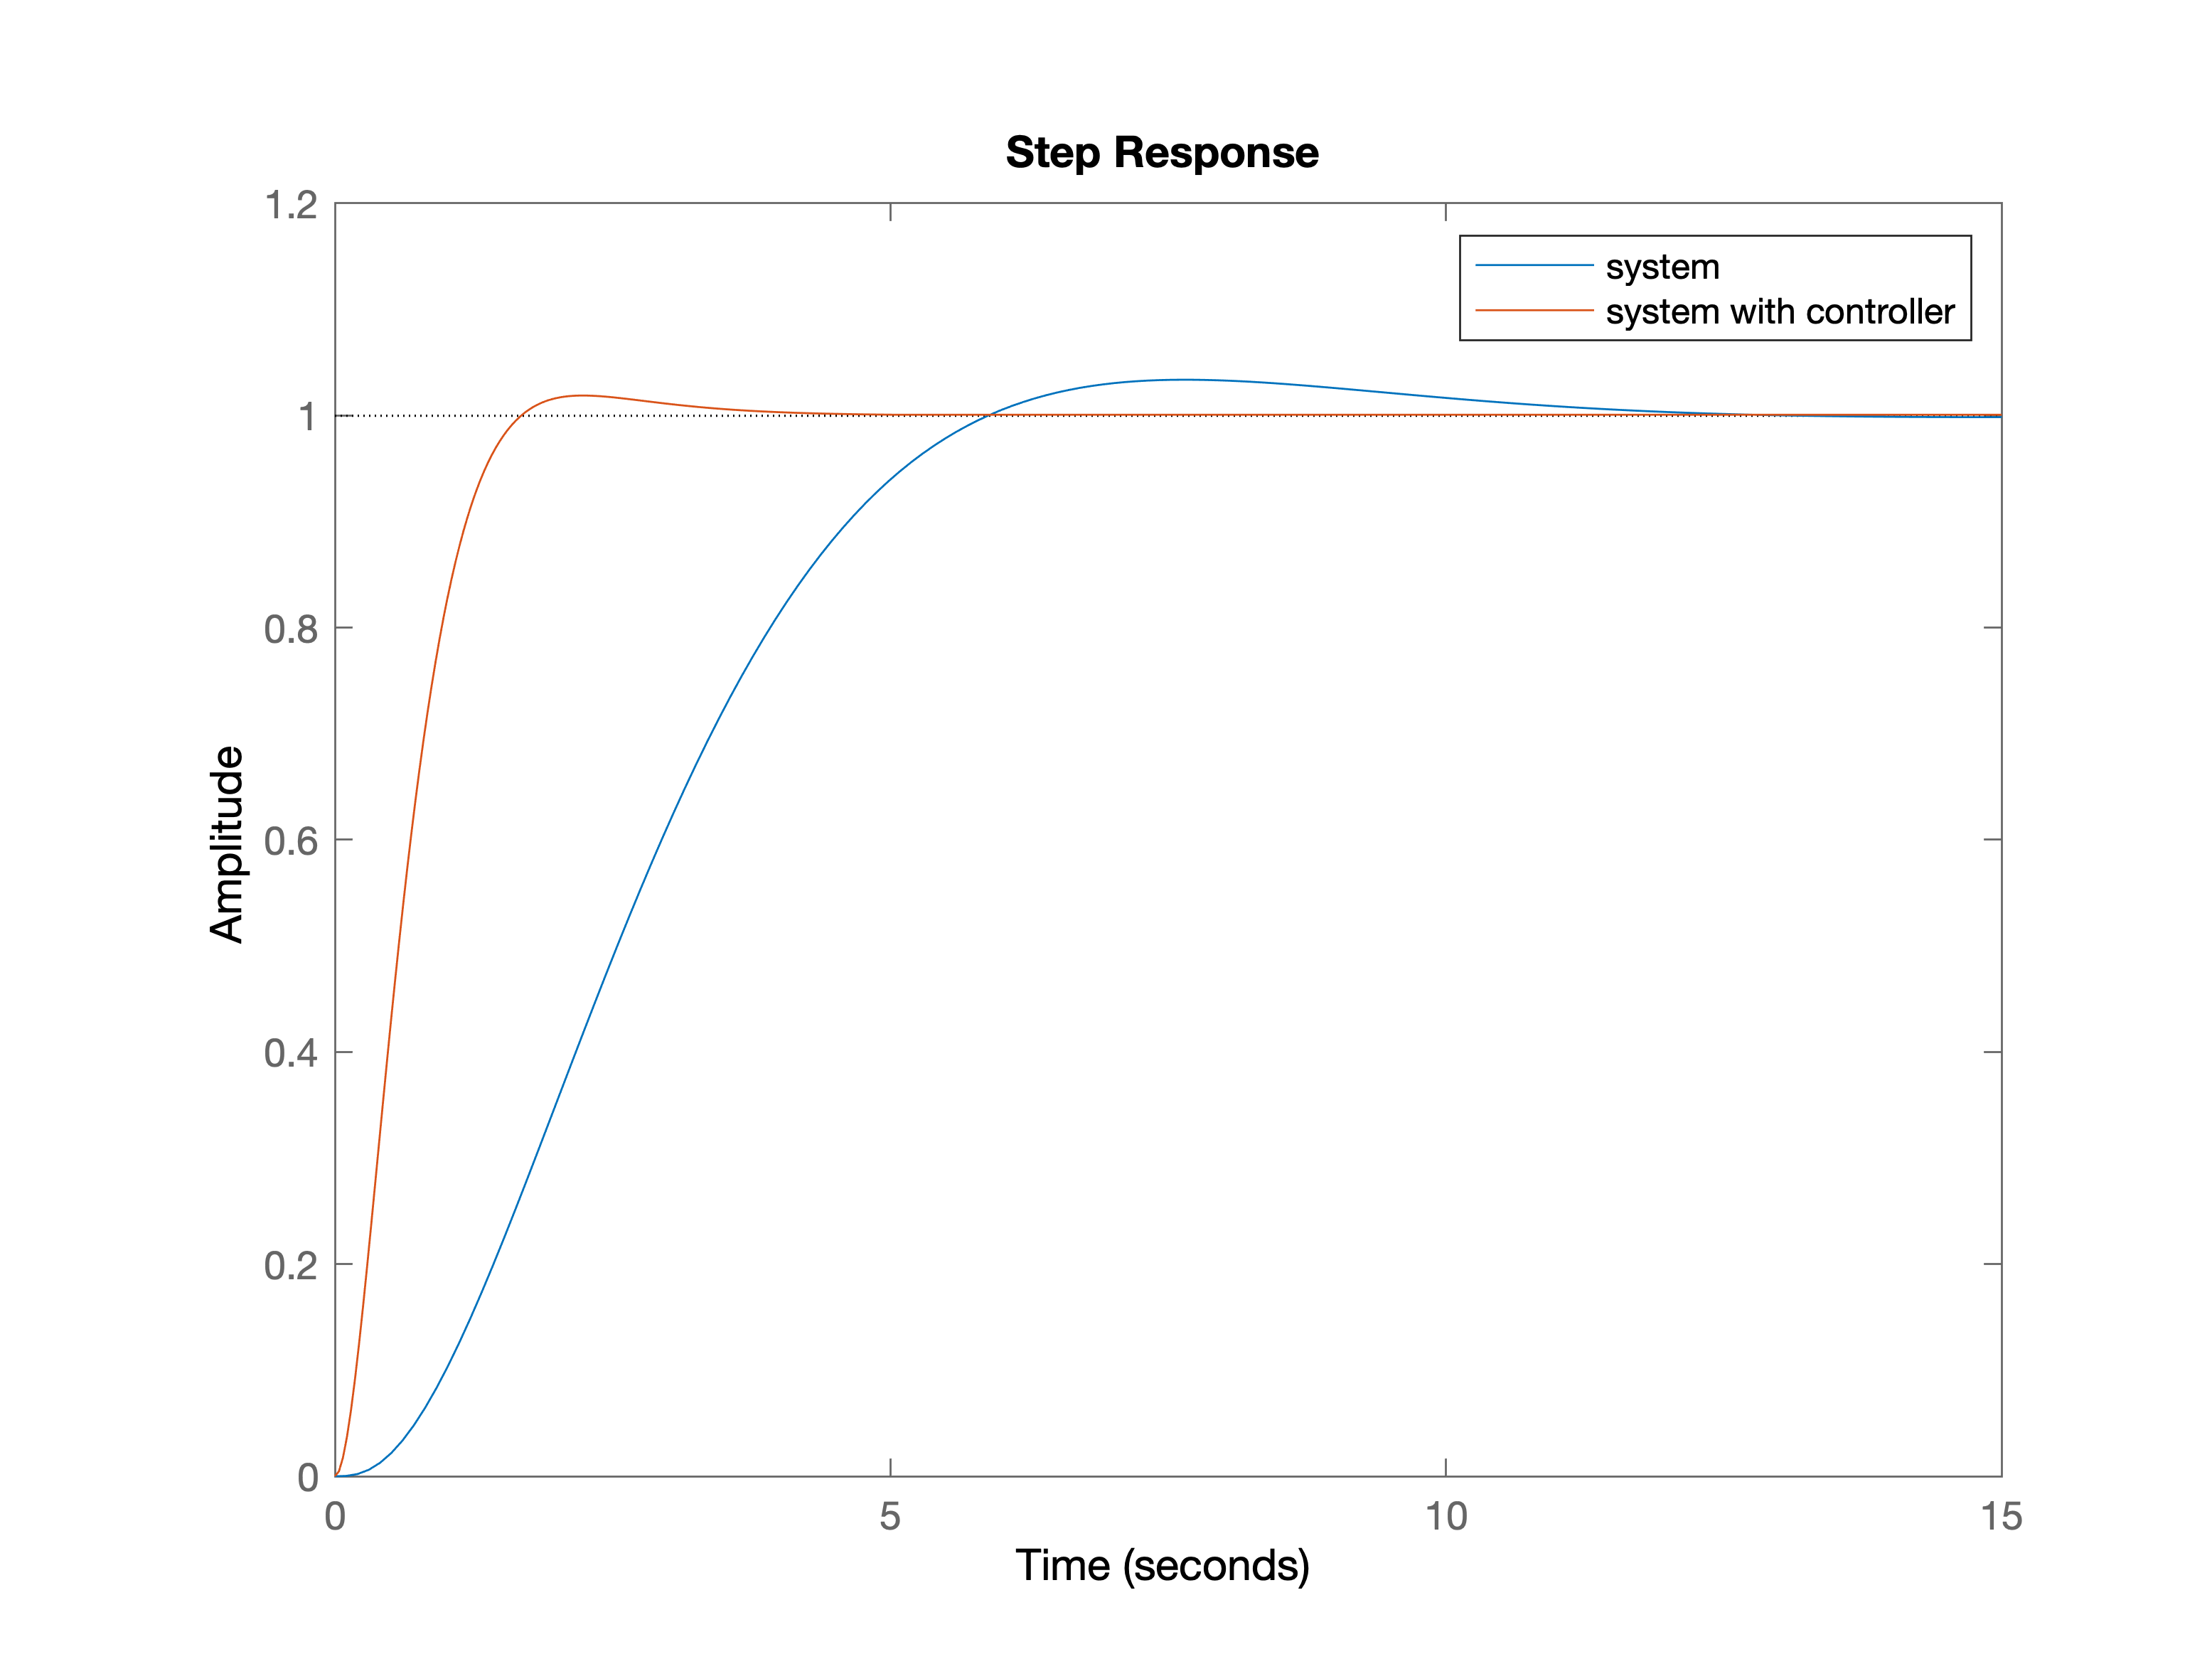
\includegraphics[width=12cm]{../Figure/Q4/Q4_respond_all.png}
    \end{figure}
    \item system with and without controller rlocus
    \begin{figure}[H]
        \caption{system with and withou controller rlocus plot}
        \centering
        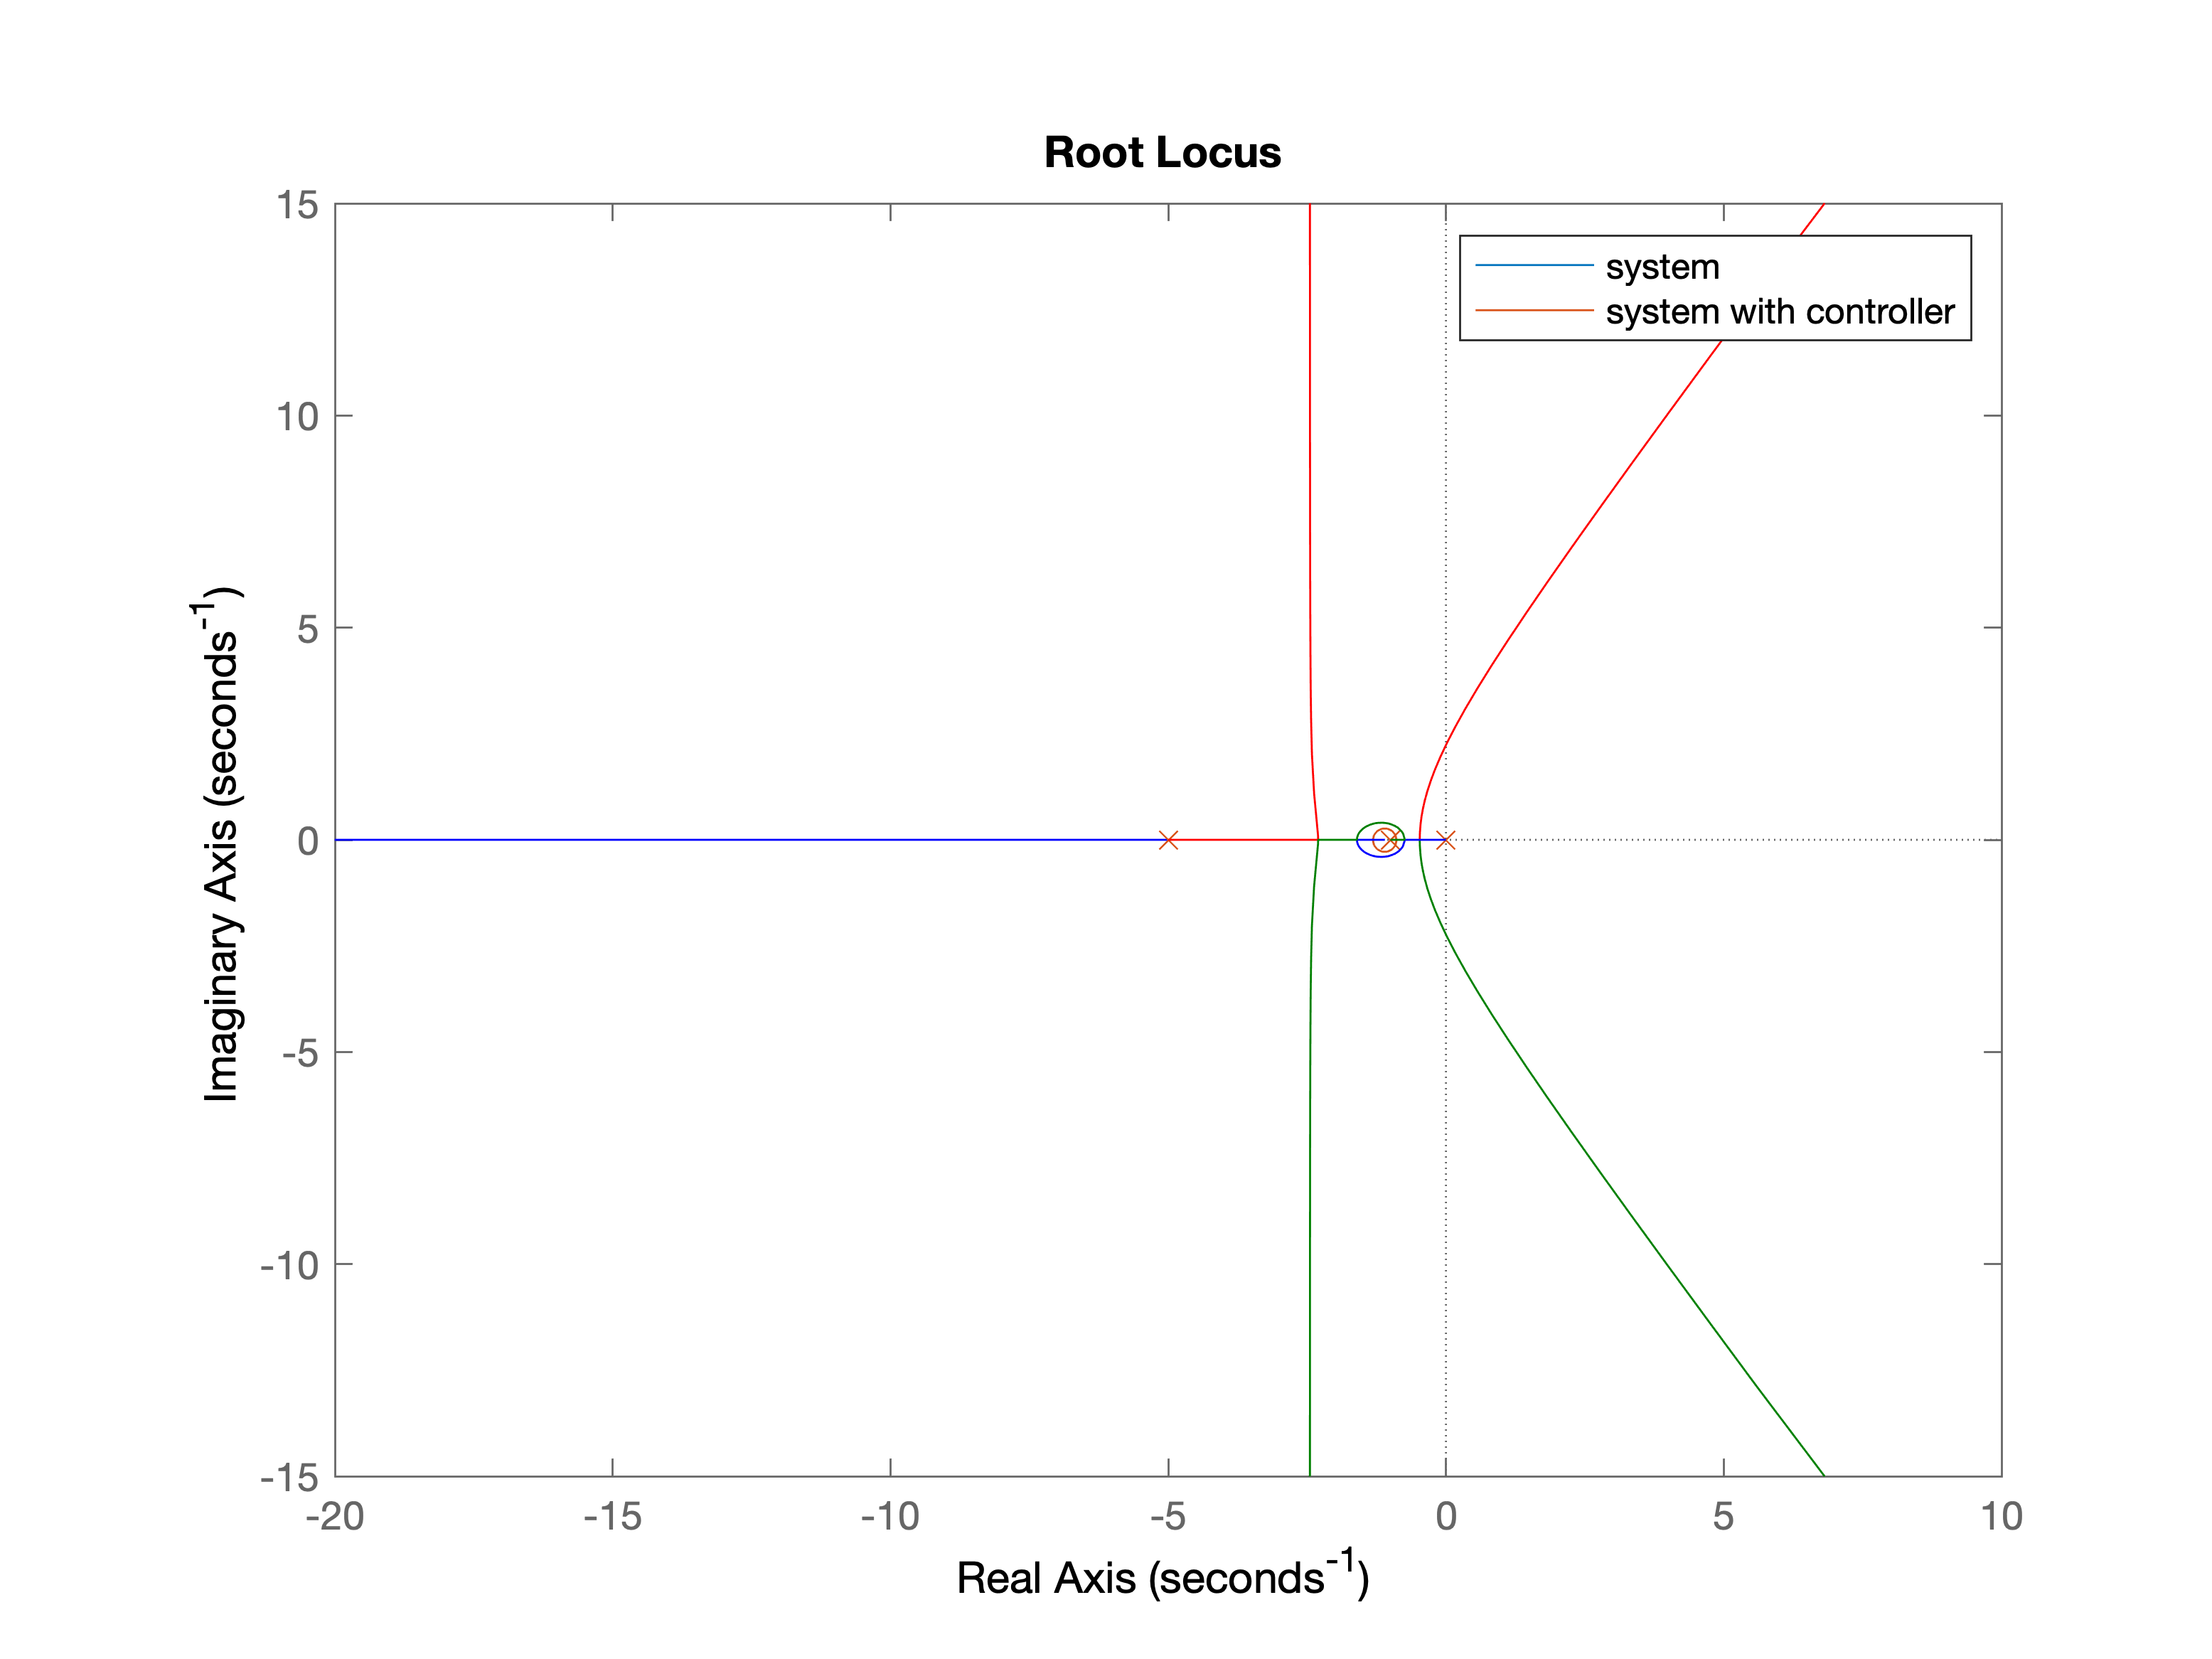
\includegraphics[width=12cm]{../Figure/Q4/Q4_rlocus.png}
    \end{figure}
\end{itemize}